\documentclass{article}

\usepackage[T1]{fontenc}    %Schriftart des Dokumentes
\usepackage[ngerman]{babel} %Dokumentensprache, hier Deutsch
\usepackage{amsmath, amssymb, stmaryrd} %mathematische Schriftzeichen
\usepackage{graphicx} %Einfügen von Grafiken
\usepackage{wrapfig}
\usepackage{bm}

\setlength{\parindent}{0pt} %Einrückung von Absätzen auf null gesetzt
\setlength{\parskip}{10pt} %Abstand zischen Absätzen auf 10pt gesetzt

\title{Versuch 26: Bestimmung der Schallgeschwindigkeit}
\author{Matthias Kuntz}
\date{04.09.2023}

\begin{document}

\maketitle

%-------------------------EINLEITUNG-------------------------
\section{Einleitung}

In diesem Versuch soll auf zwei verschiedene Wege die Schallgeschwindigkeit in Luft und in Kohlenstoffdioxid bestimmt werden, einmal mit einem Quinke’schen Rohr und einmal mit einem Aufbau mit Oszilloskop. Beim ersten Versuch kann die Höhe des Reflektors des Quinke'schen Rohrs, was hier die Oberfläche einer Wassersäule im Rohr ist, verändert werden, sodass Lautstärkemaxima und -minima enstehen. Mit Angaben über die effektive Länge des Rohres bei diesen Stellen kann dann die Schallgeschwindigkeit bestimmt werden.

Der zweite Versuch sieht die Messung der Laufzeit einer Schallwelle in der Luft mithilfe eines Oszilloskops sowie einem Lautsprecher und einem Mikrofon vor. Die Schallgeschwindigkeit wird hier über die Differenz der gemessenen Werte bestimmt.

\subsection{Versuchsaufbau}

Für diesen Versuch werden zwei verschiede Versuchsaufbauten verwendet, die in Abbildung \ref{gr:N1} und \ref{gr:N2} dargestellt sind.

Beim ersten Versuch wird über einen Lautsprecher eine Sinuswelle in ein Glasrohr geleitet, welches unten mit Wasser befüllt ist. Der Wasserspiegel ist in der Höhe veränderlich. Hört man über das oben am Glasrohr angebrachte Stehtoskop das Signal der Sinuswelle im Rohr ab so stellt man fest, dass sich die Lautstärke abhängig von der Höhe des Wasserspiegels verändert. Zum Ablesen der Wasserhöhe ist ein Maßstab neben dem Rohr angebracht.

\begin{figure}[h] 
\centering
\caption{Versuchsaufbau 1 mit Quinke'schem Rohr}
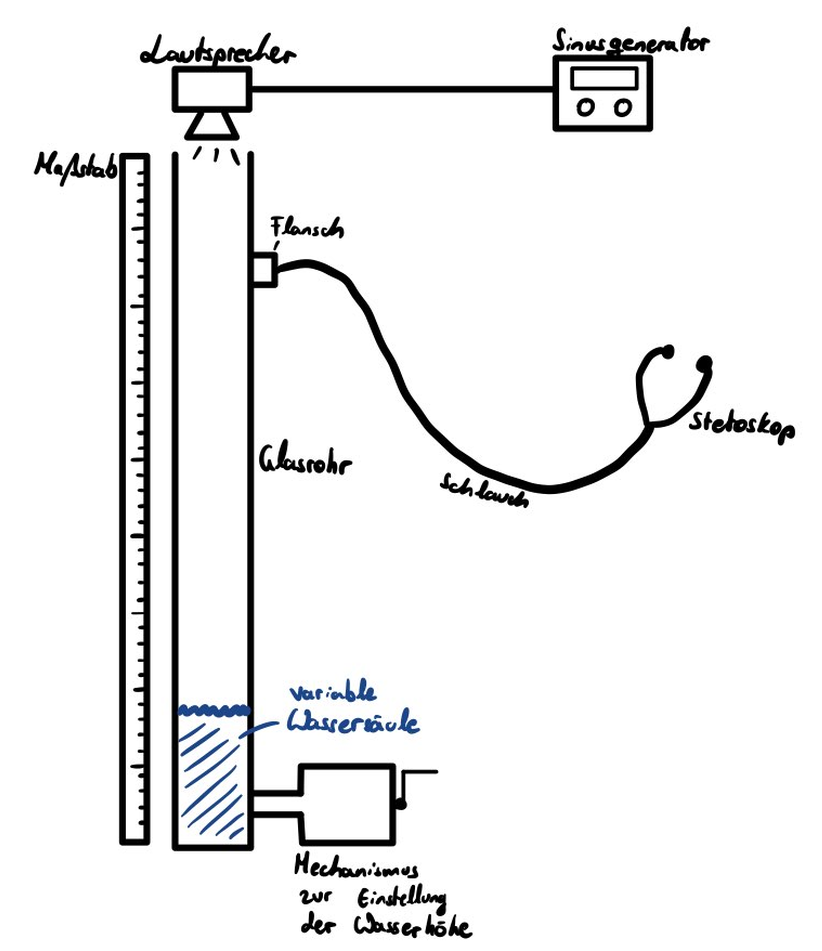
\includegraphics[width=6cm]{graphics/Skizze1.png} \label{gr:N1}
\end{figure}

\newpage 

Beim zweiten Versuch sendet ein Sinusgenerator eine Sinuswelle einmal direkt an ein Oszilloskop und gleichzeitig an einen Lautsprecher, welcher das Signal als Ton zu einem höhenverstellbaren Mikrofon schickt. Das Eingangssignal vom Mikrofon wird an einen zweiten Kanal des Oszilloskops angeschlossen. Verstellt man die Höhe des Mikrofons, ergo den Abstand zwischen Lautsprecher und Mikrofon, so kann man eine Phasenverschiebung der vom Mirkofon aufgenommenen Welle auf dem Oszilloskop beobachten. Es ist ein Maßstab zum Ablesen der Höhe des Mikrofons angebracht.

\begin{figure}[h] 
\centering
\caption{Versuchsaufbau 2 mit Oszilloskop} \label{gr:N2}
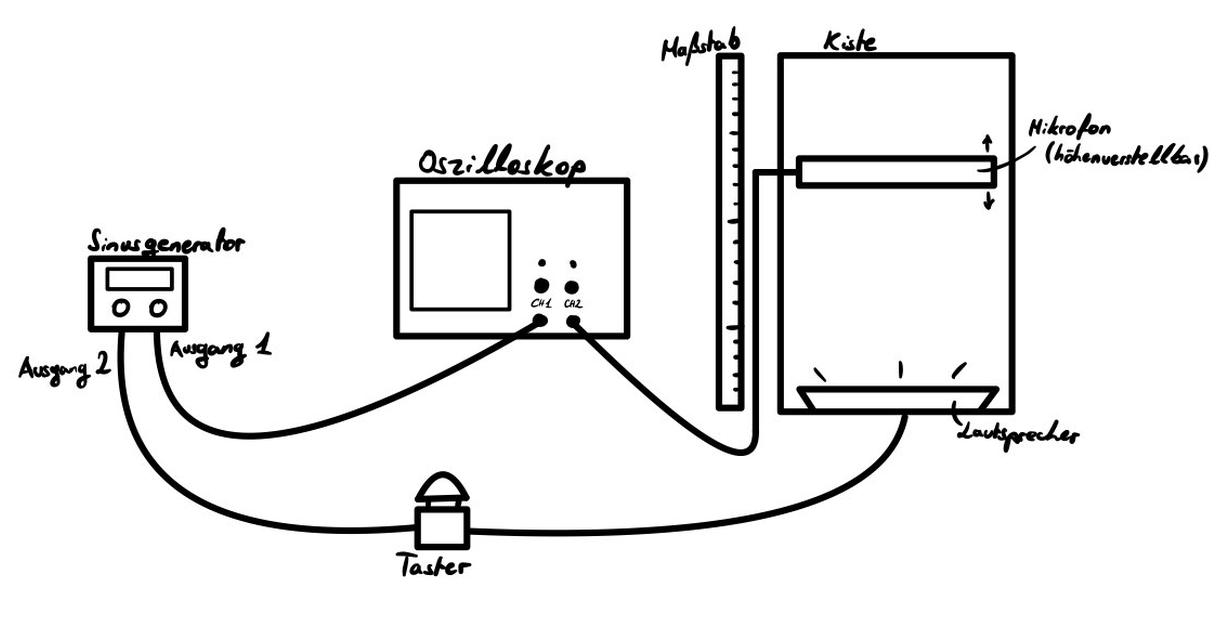
\includegraphics[width=6cm]{graphics/Skizze2.png}
\end{figure}

\newpage

\subsection{Physikalische Grundlagen}

Da Wellen ein großer Bestandteil dieses Versuchs sind, sollen nun zuerst diese grundlegend erläutert werden.

Als Wellen bezeichnet man räumliche und zeitliche Zustandsänderungen physikalischer Größen, die häufig nach festen periodischen Regeln erfolgen. Bei Wellen unterscheidet man vor allem zwischen zwei Typen, den longitudinalen und den transversalen Wellen. Transversalwellen sind solche, bei denen die Welle senkrecht zur Ausbreitungsrichtung schwingt, während Longitudinalwellen in ihre Ausbreitungsrichtung schwingen.

Ein weiterer Begriff ist der der sogenannten stehenden Welle. Eine stehende Welle entsteht bei der Überlagerung zweier gegeneinander laufenden Wellen gleicher Frequenz und Amplitude. Dieses Phänomen entsteht beispielsweise bei der Reflexion einer Welle, indem der reflektierte Teil mit dem einfallenden interferiert - so wird auch im ersten Teil dieses Versuches eine stehende Welle erzeugt. Die Besonderheit einer stehenden Welle ist, dass sich die Positionen der Punke minimaler und maximaler Auslenkung nicht verändern. Es entstehen also Fixpunkte, die immer eine Auslenkung von 0 haben, und somit wirkt die Welle, als würde sie stehen. 

\begin{wrapfigure}{l}{0.25\textwidth}
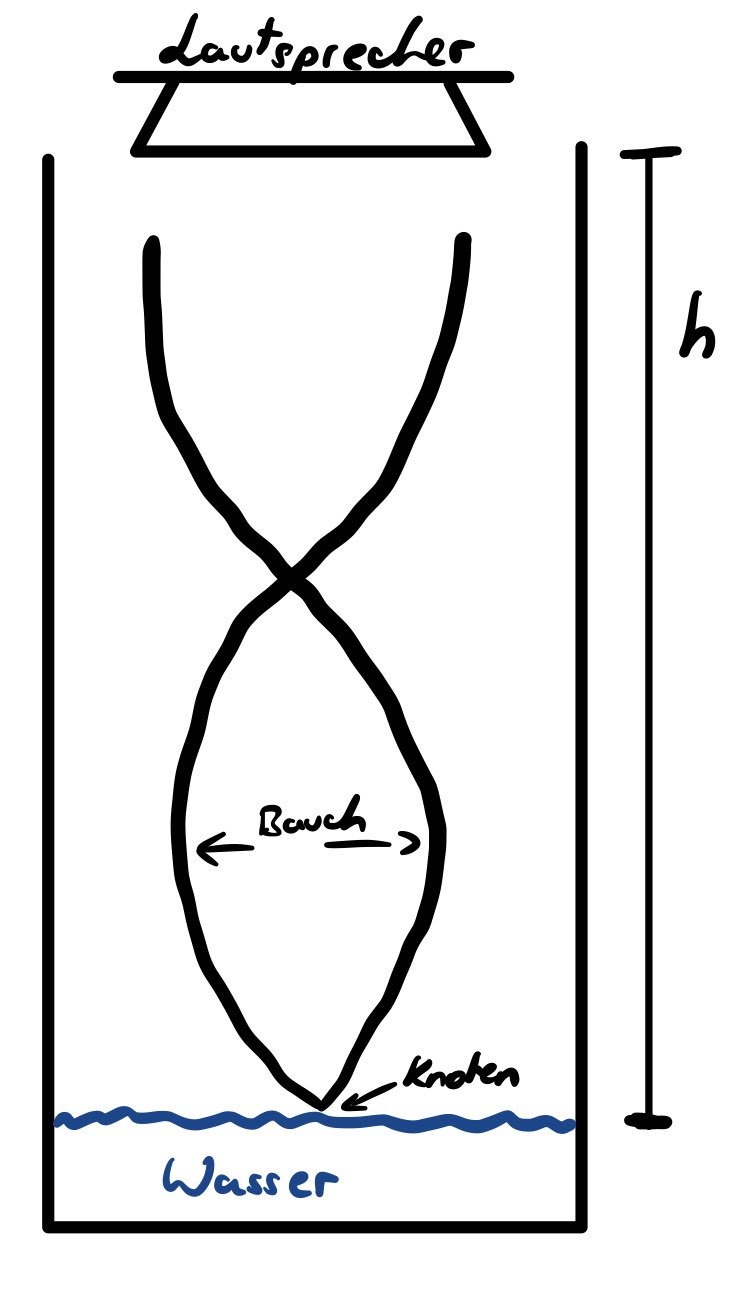
\includegraphics[width=0.9\linewidth]{graphics/Skizze1-1.jpg} 
\caption{Stehende Welle im Quinke'schen Rohr}
\label{fig:wrapfig}
\end{wrapfigure}

Erzeugt man wie im ersten Versuch eine stehende Welle in einem Rohr, so hat diese beim Lautsprecher einen Wellenbauch und am Reflektor, in diesem Fall der Wasseroberfläche, einen Wellenknoten. Im Resonanzfall, ergo einem Lautstärkemaximum, muss für die effektive Höhe $h$ des Rohrs dann gelten

\begin{equation}
    h=\frac{2n+1}{4} \lambda . \label{fr:N1}
\end{equation}

Wobei hier $\lambda$ für die Wellenlänge der Welle steht und \\ $n \in \mathbb{N}$ ist.

Mit Gleichung (1) lässt sich also die Differenz $D$ zwischen zwei Lautstärkemaxima bestimmen:

\begin{equation}
    D=h_{n+1} - h_{n} = \frac{2(n+1)+1}{4} \lambda - \frac{2n+1}{4} \lambda = \frac{\lambda}{2} \label{fr:N2}
\end{equation}

Um im Endeffekt die Schallgeschwindigkeit $c$ zu berechnen verwendet man den Zusammenhang $c=\lambda \nu$, wobei $\nu$ die Frequenz der Welle ist, und erhält somit in Verbindung mit Gleichung (2):

\begin{equation}
    c=\nu \lambda = 2 \nu D \label{fr:N3} 
\end{equation}

Ein alternativer Weg zur Berechnung der Schallgeschindigkeit läuft über die Formel für die Schallgeschindigkeit in Gasen:

\begin{equation}
    c = \sqrt{\frac{\kappa R T}{M}} \label{fr:N4}
\end{equation}

Hierbei steht $\kappa$ für den Adiabatenkoeffizienten (für Luft $\kappa = 1,40$, für $CO_2$ $\kappa = 1,30$), $R$ für die allgemeine Gaskonstante, $T$ die Temperatur des Gases in Kelvin und $M$ die Molekülmasse (für Luft $M=29g/mol$, für $CO_2$ $M=44g/mol$).

Wenn wir später die Schallgeschwindigkeiten bestimmt haben, sind diese in Abhängigkeit von der Raumtemperatur. Um sie auf die Normalbedingung von $T_0 = 273,15^{\circ}K$ umzurechnen verwendet man die Gleichung:

\begin{equation}
    \frac{c_0}{c} = \sqrt{\frac{T_0}{T}} \label{fr:N5}
\end{equation}

Hier sind $T$ und $c$ die von uns bestimmten Werte und $c_0$ ist der Wert bei Normalbedingungen.

Beim zweiten Versuch muss die Sinuswelle die Distanz zwischen Lautsprecher und Mikrofon zurücklegen, bevor sie am Oszilloskop ankommt. Die Zeit $\tau$, die die Schallwelle braucht um diese Distanz $l$ zu überbrücken ist gegeben durch

\begin{equation}
    \tau = \frac{l}{c}
\end{equation}

Da dadurch nun eine Phasenverschiebung auf dem Oszilloskop zu erkennen ist, lässt sich der Abstand bestimmen, den man das Mikrofon verstellen muss um eine Phasenverschiebung von genau einer Periode zu verfolgen. Man kann also die Differenz $D$ des Abstands bei einer solchen Phasenverschiebung bestimmen und diese mit einer Wellenlänge identifizieren:

\begin{equation}
    l_{n+1} - l_n = D = \lambda
\end{equation}

Anschließend kann man mit Gleichung 3 die Schallgeschwindigkeit bestimmen:

\begin{equation}
    c = \nu \lambda = \nu D
\end{equation}

%---------------VERSUCHSPROTOKOLL MIT MESSDATEN---------------

\newpage

\section{Versuchsprotokoll mit Messdaten}

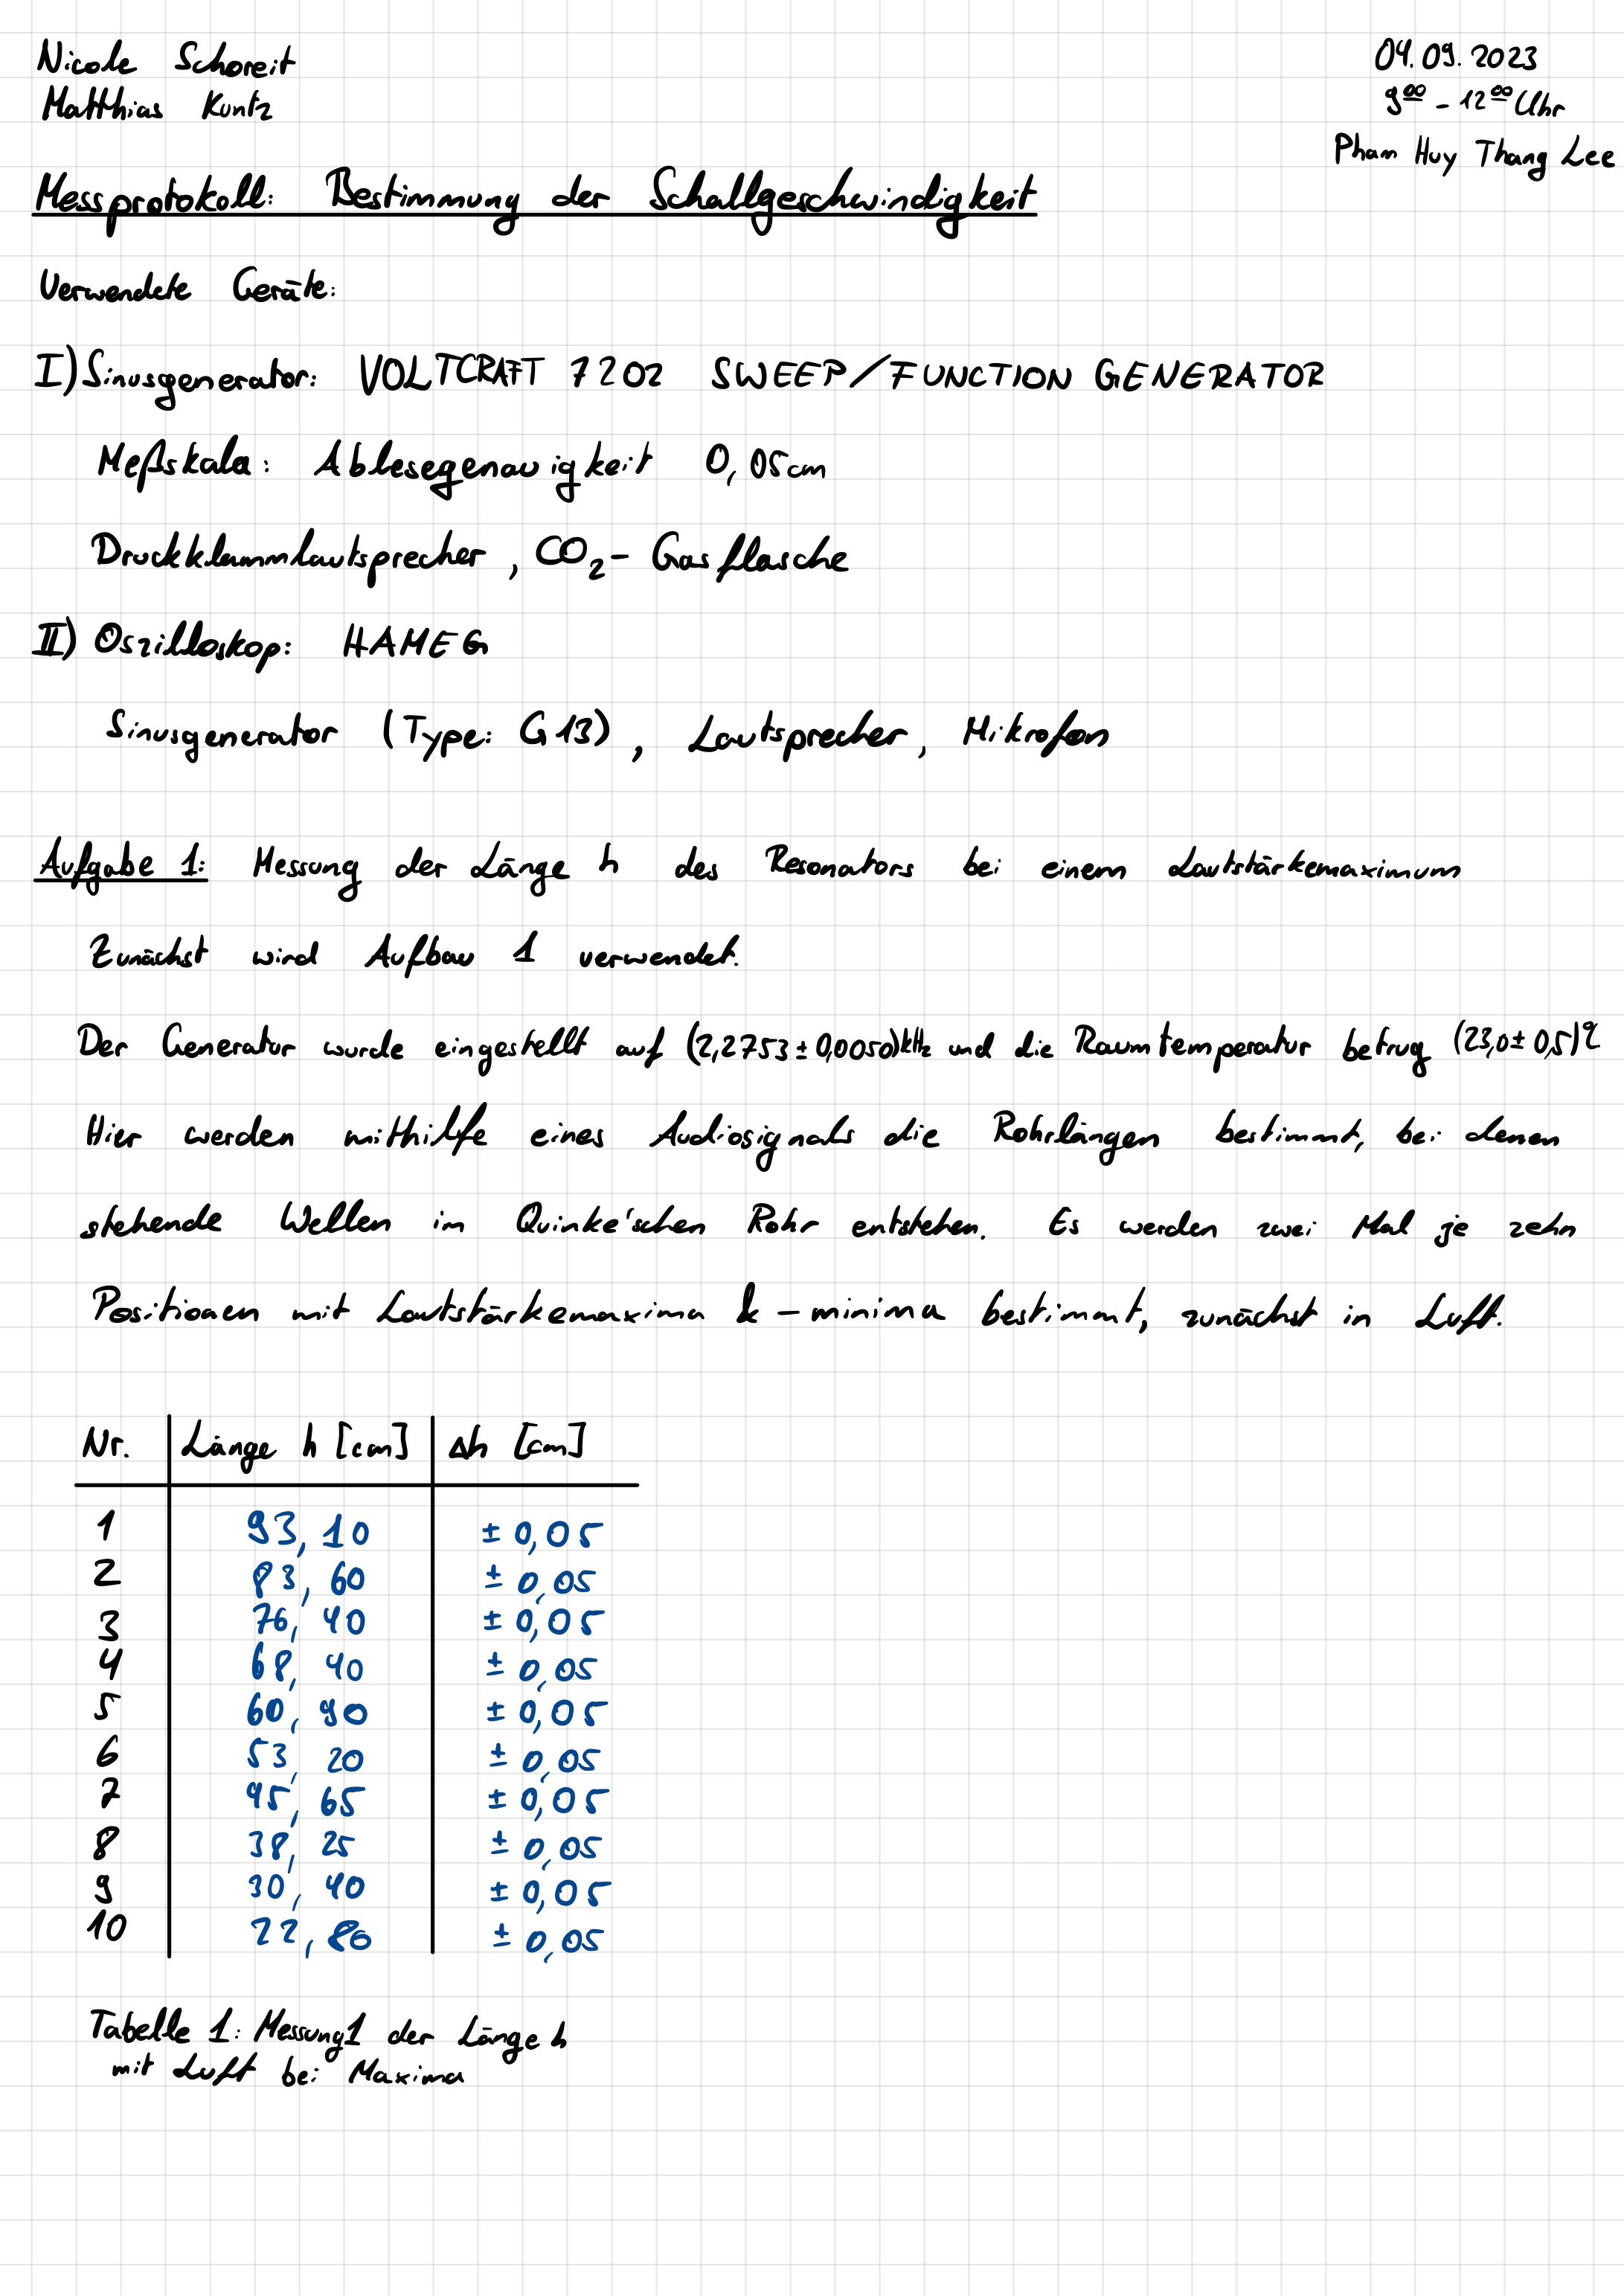
\includegraphics[width=\textwidth]{graphics/mess1.jpg}
\newpage
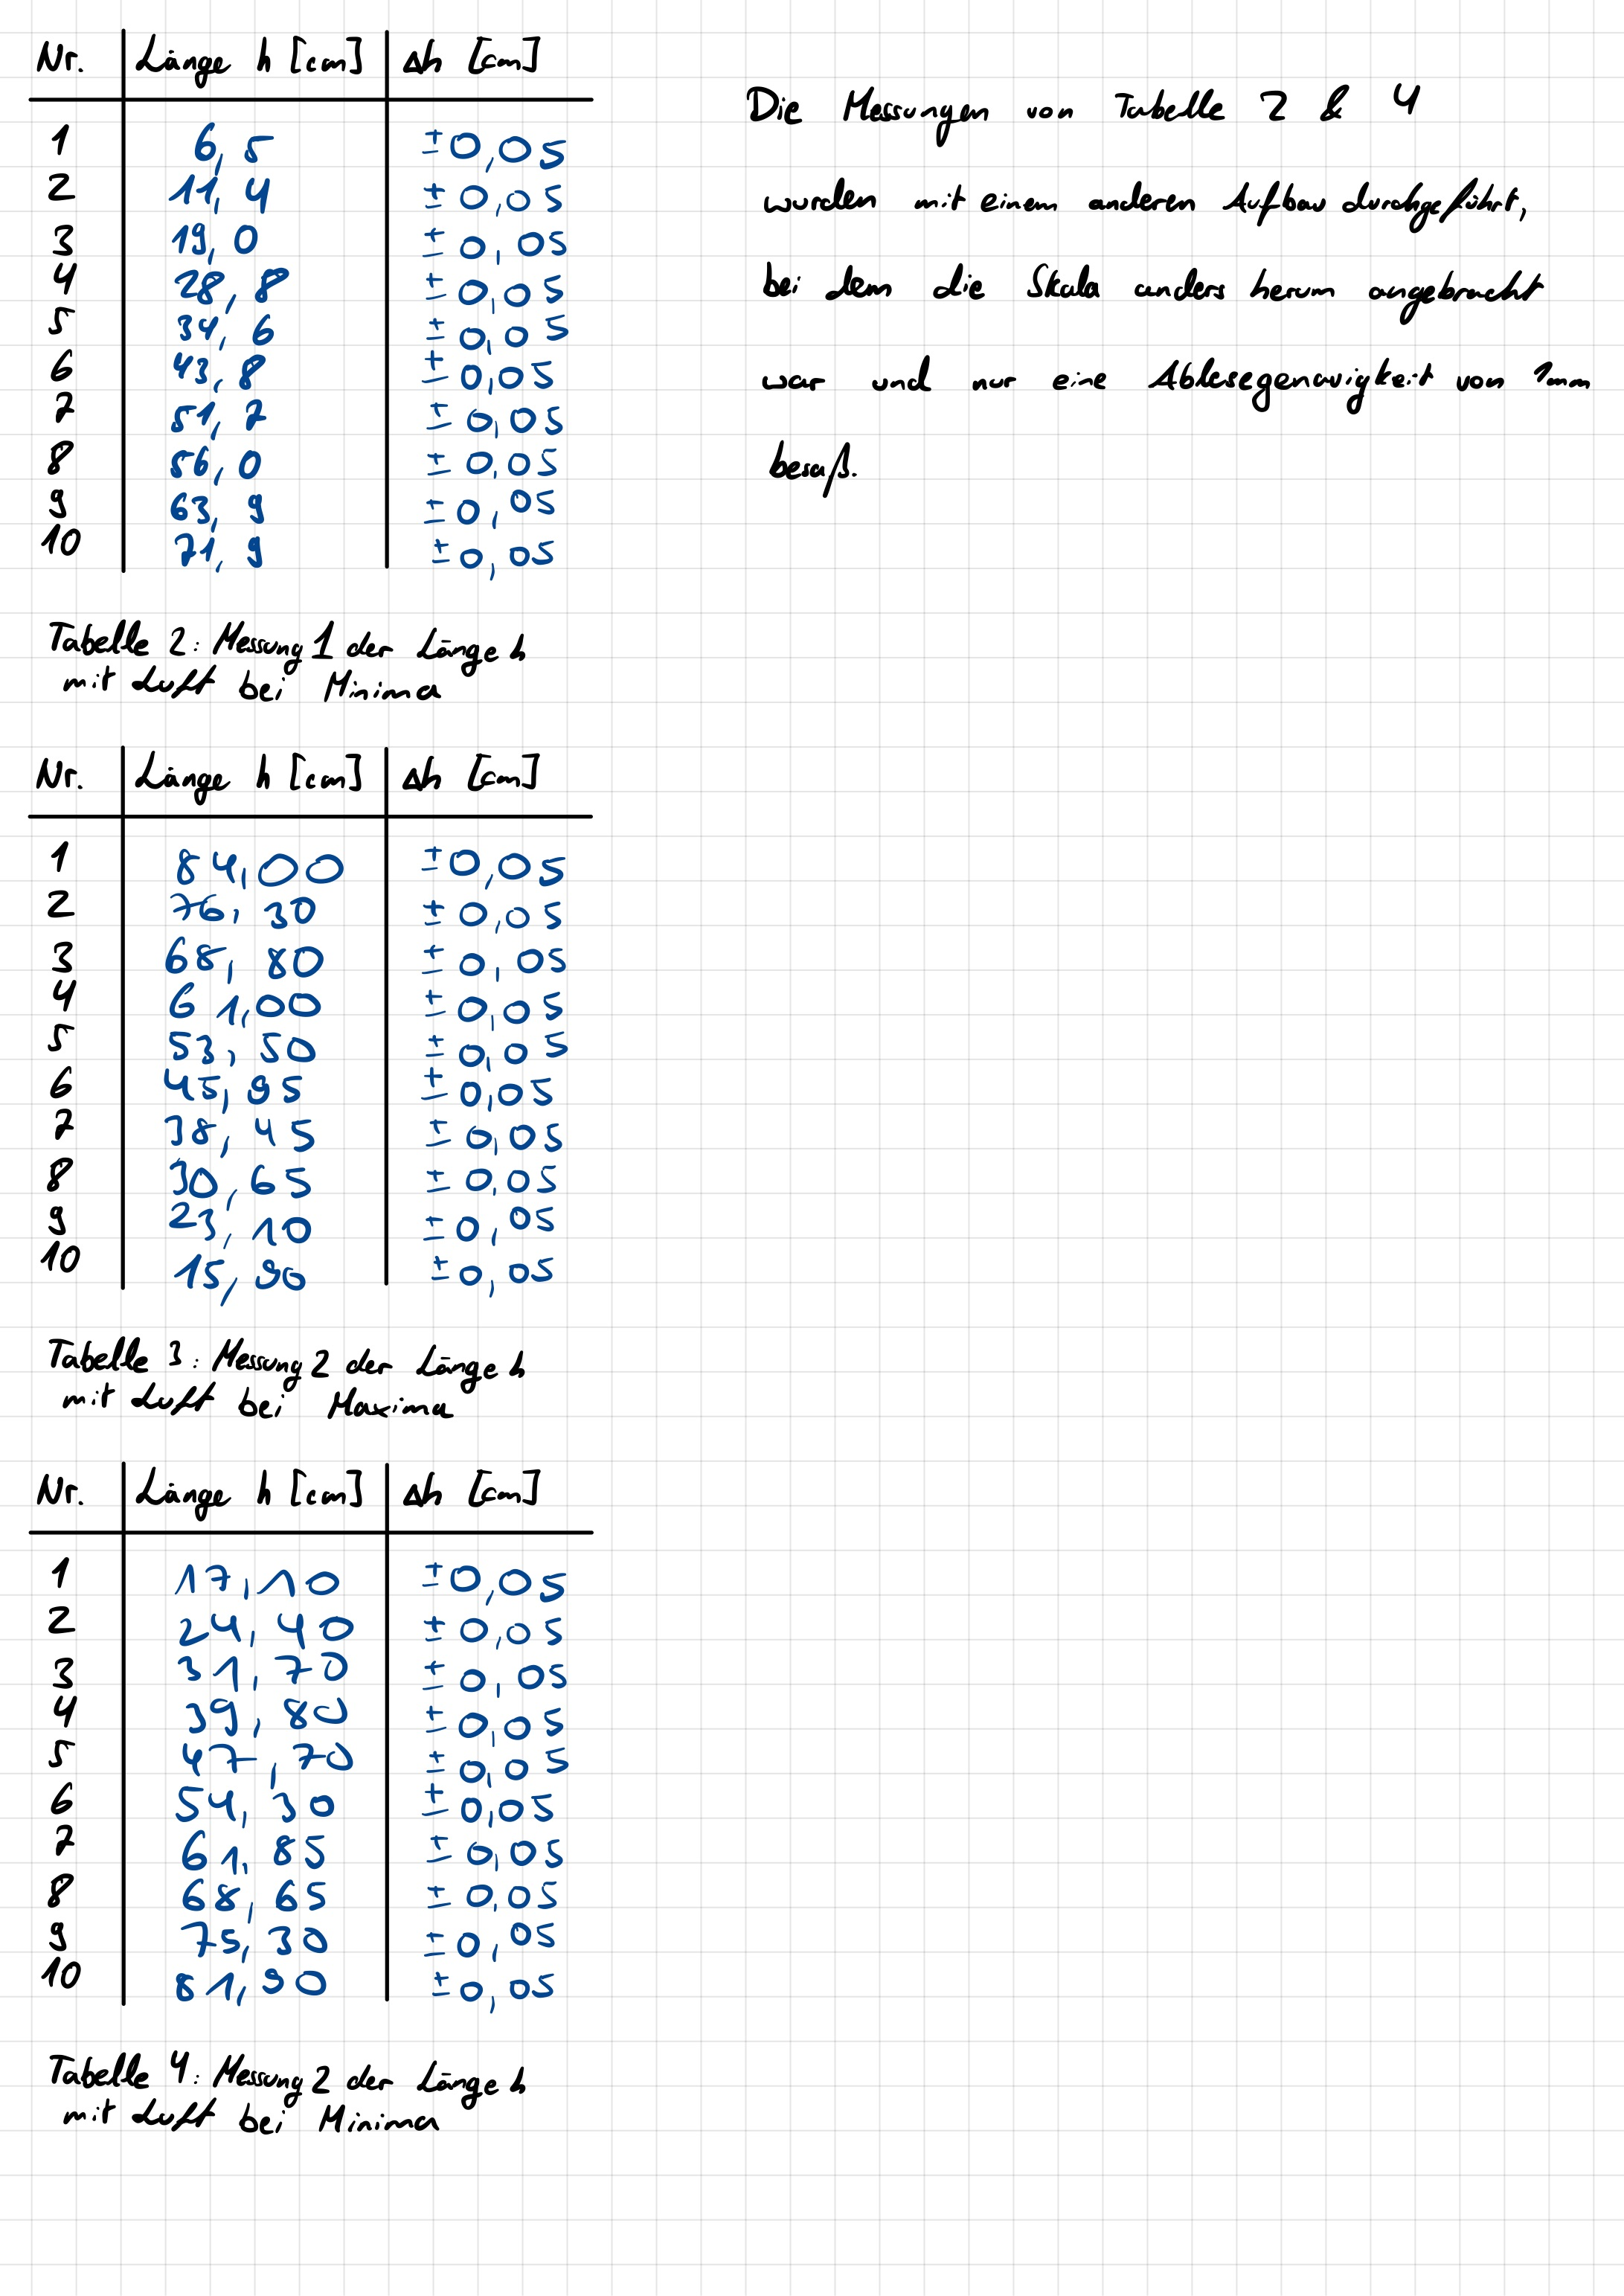
\includegraphics[width=\textwidth]{graphics/mess2.jpg}
\newpage
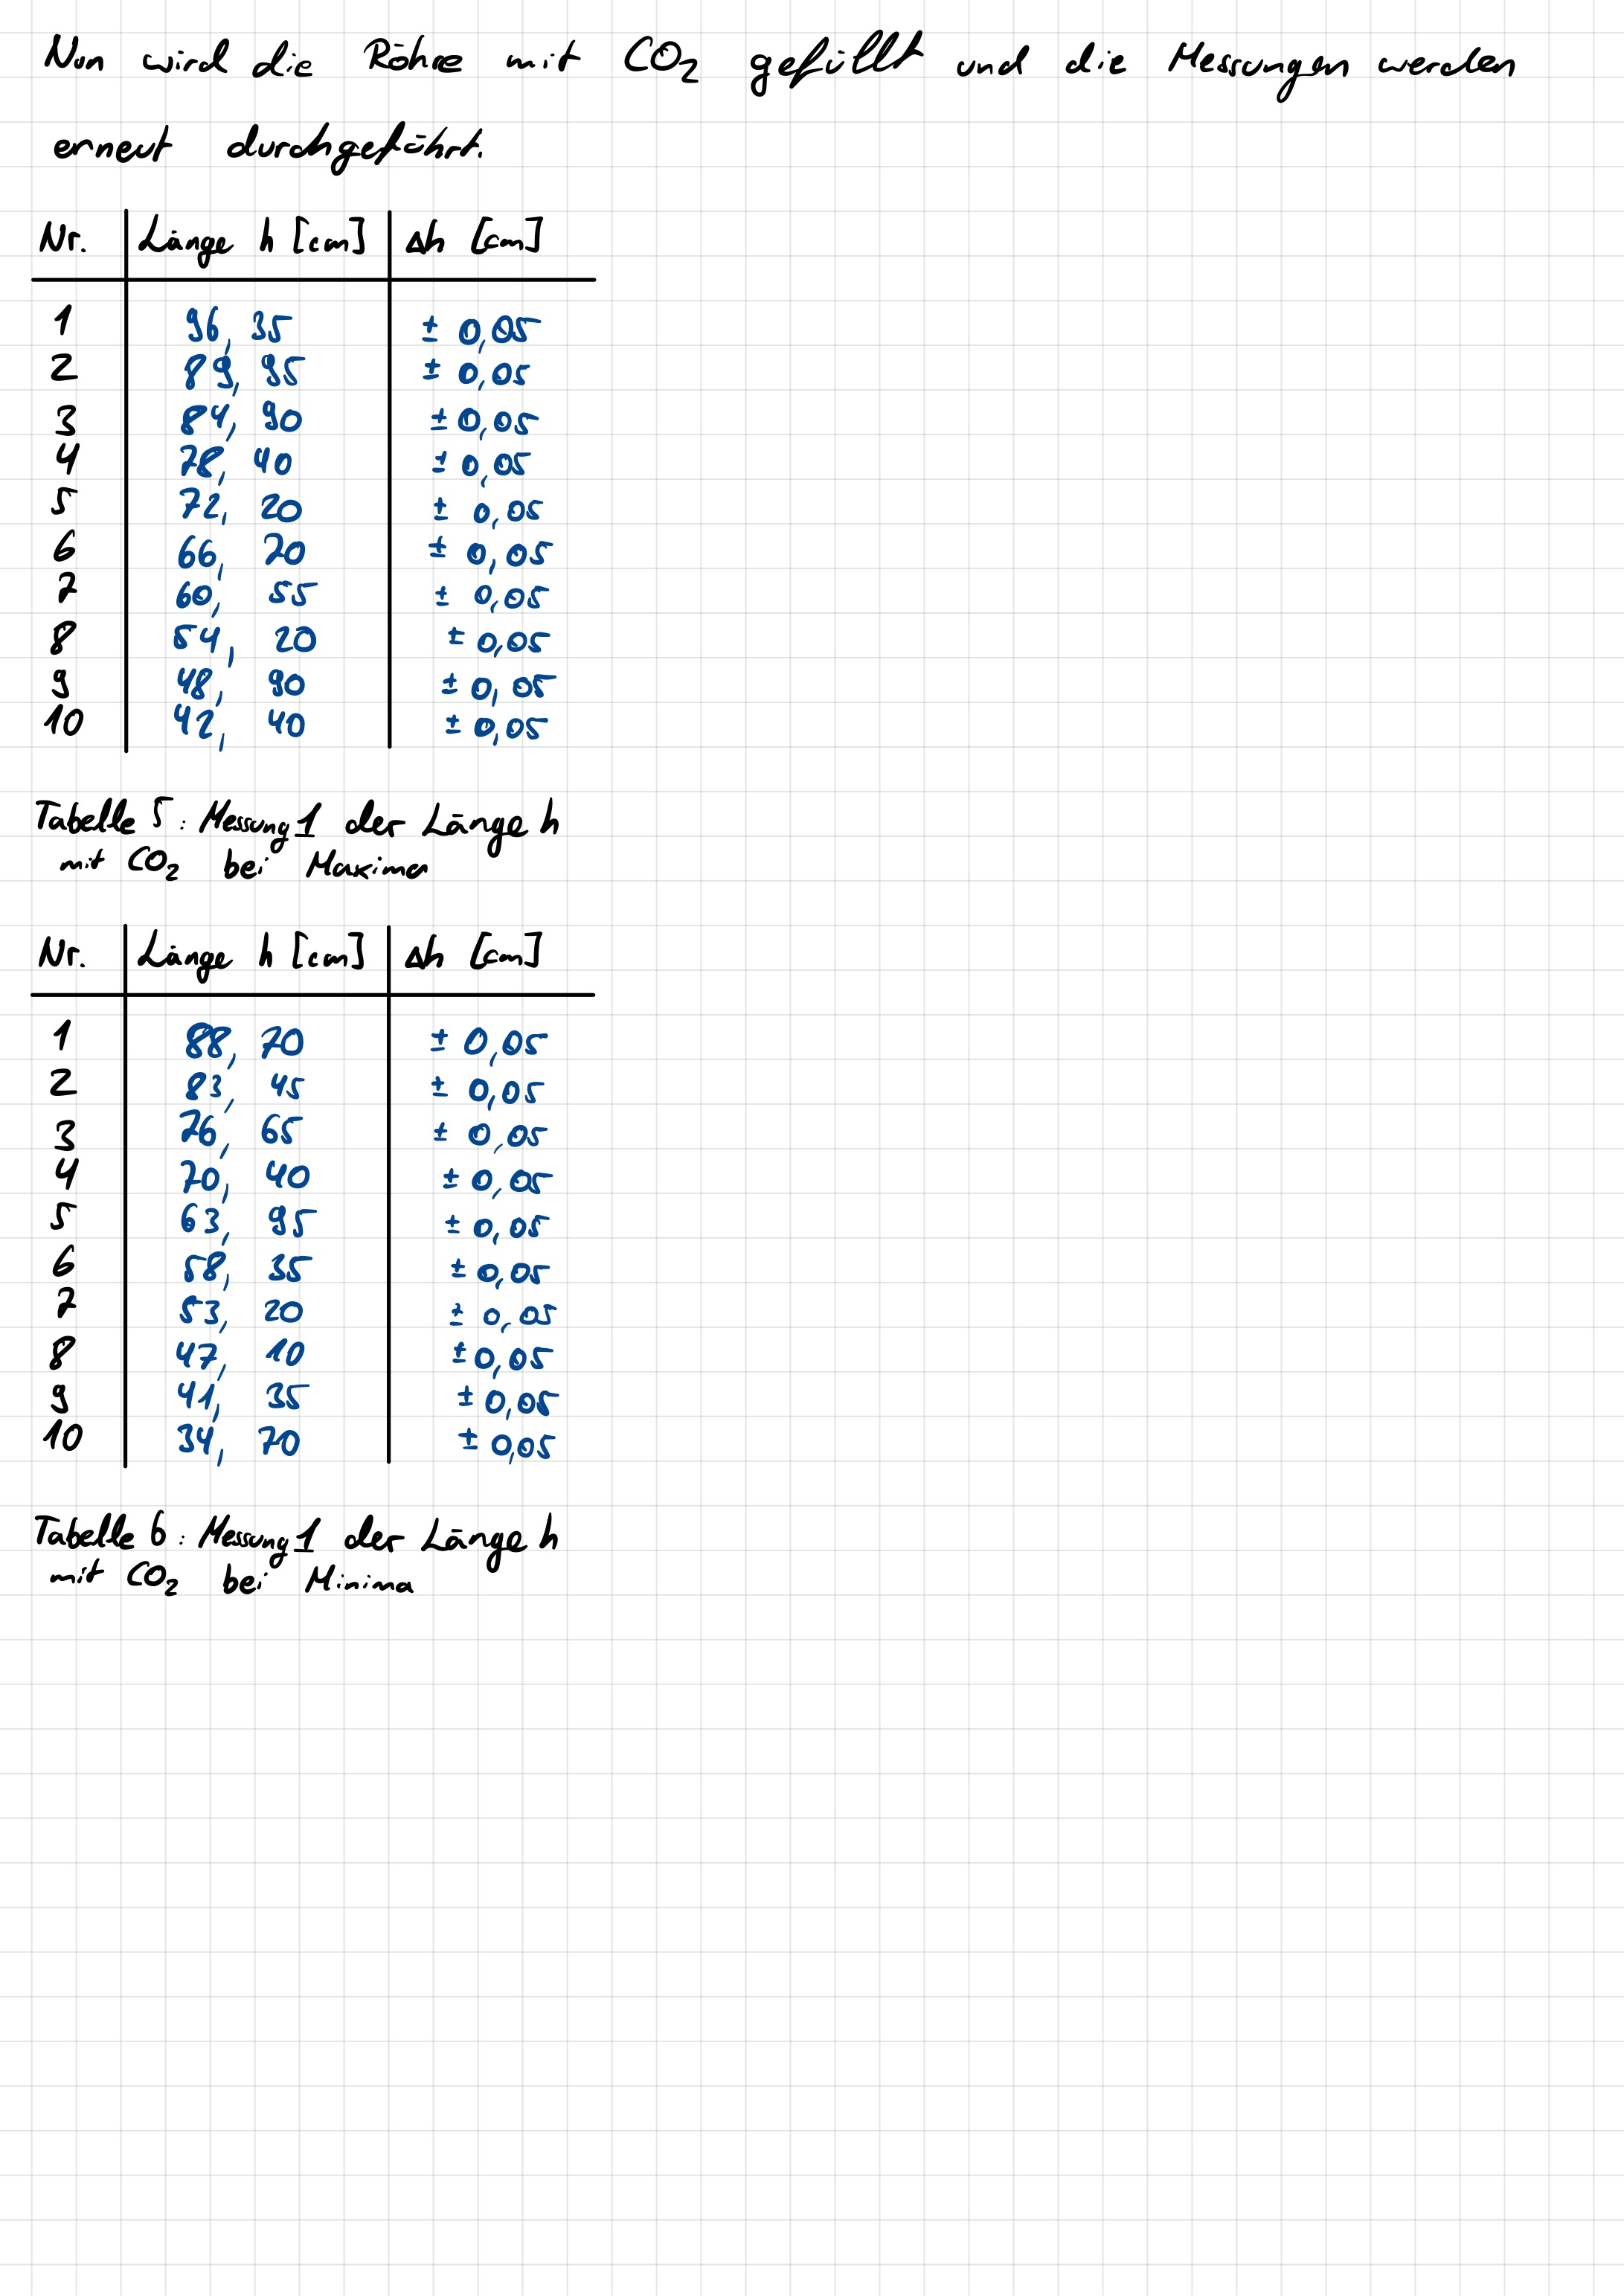
\includegraphics[width=\textwidth]{graphics/mess3.jpg}
\newpage
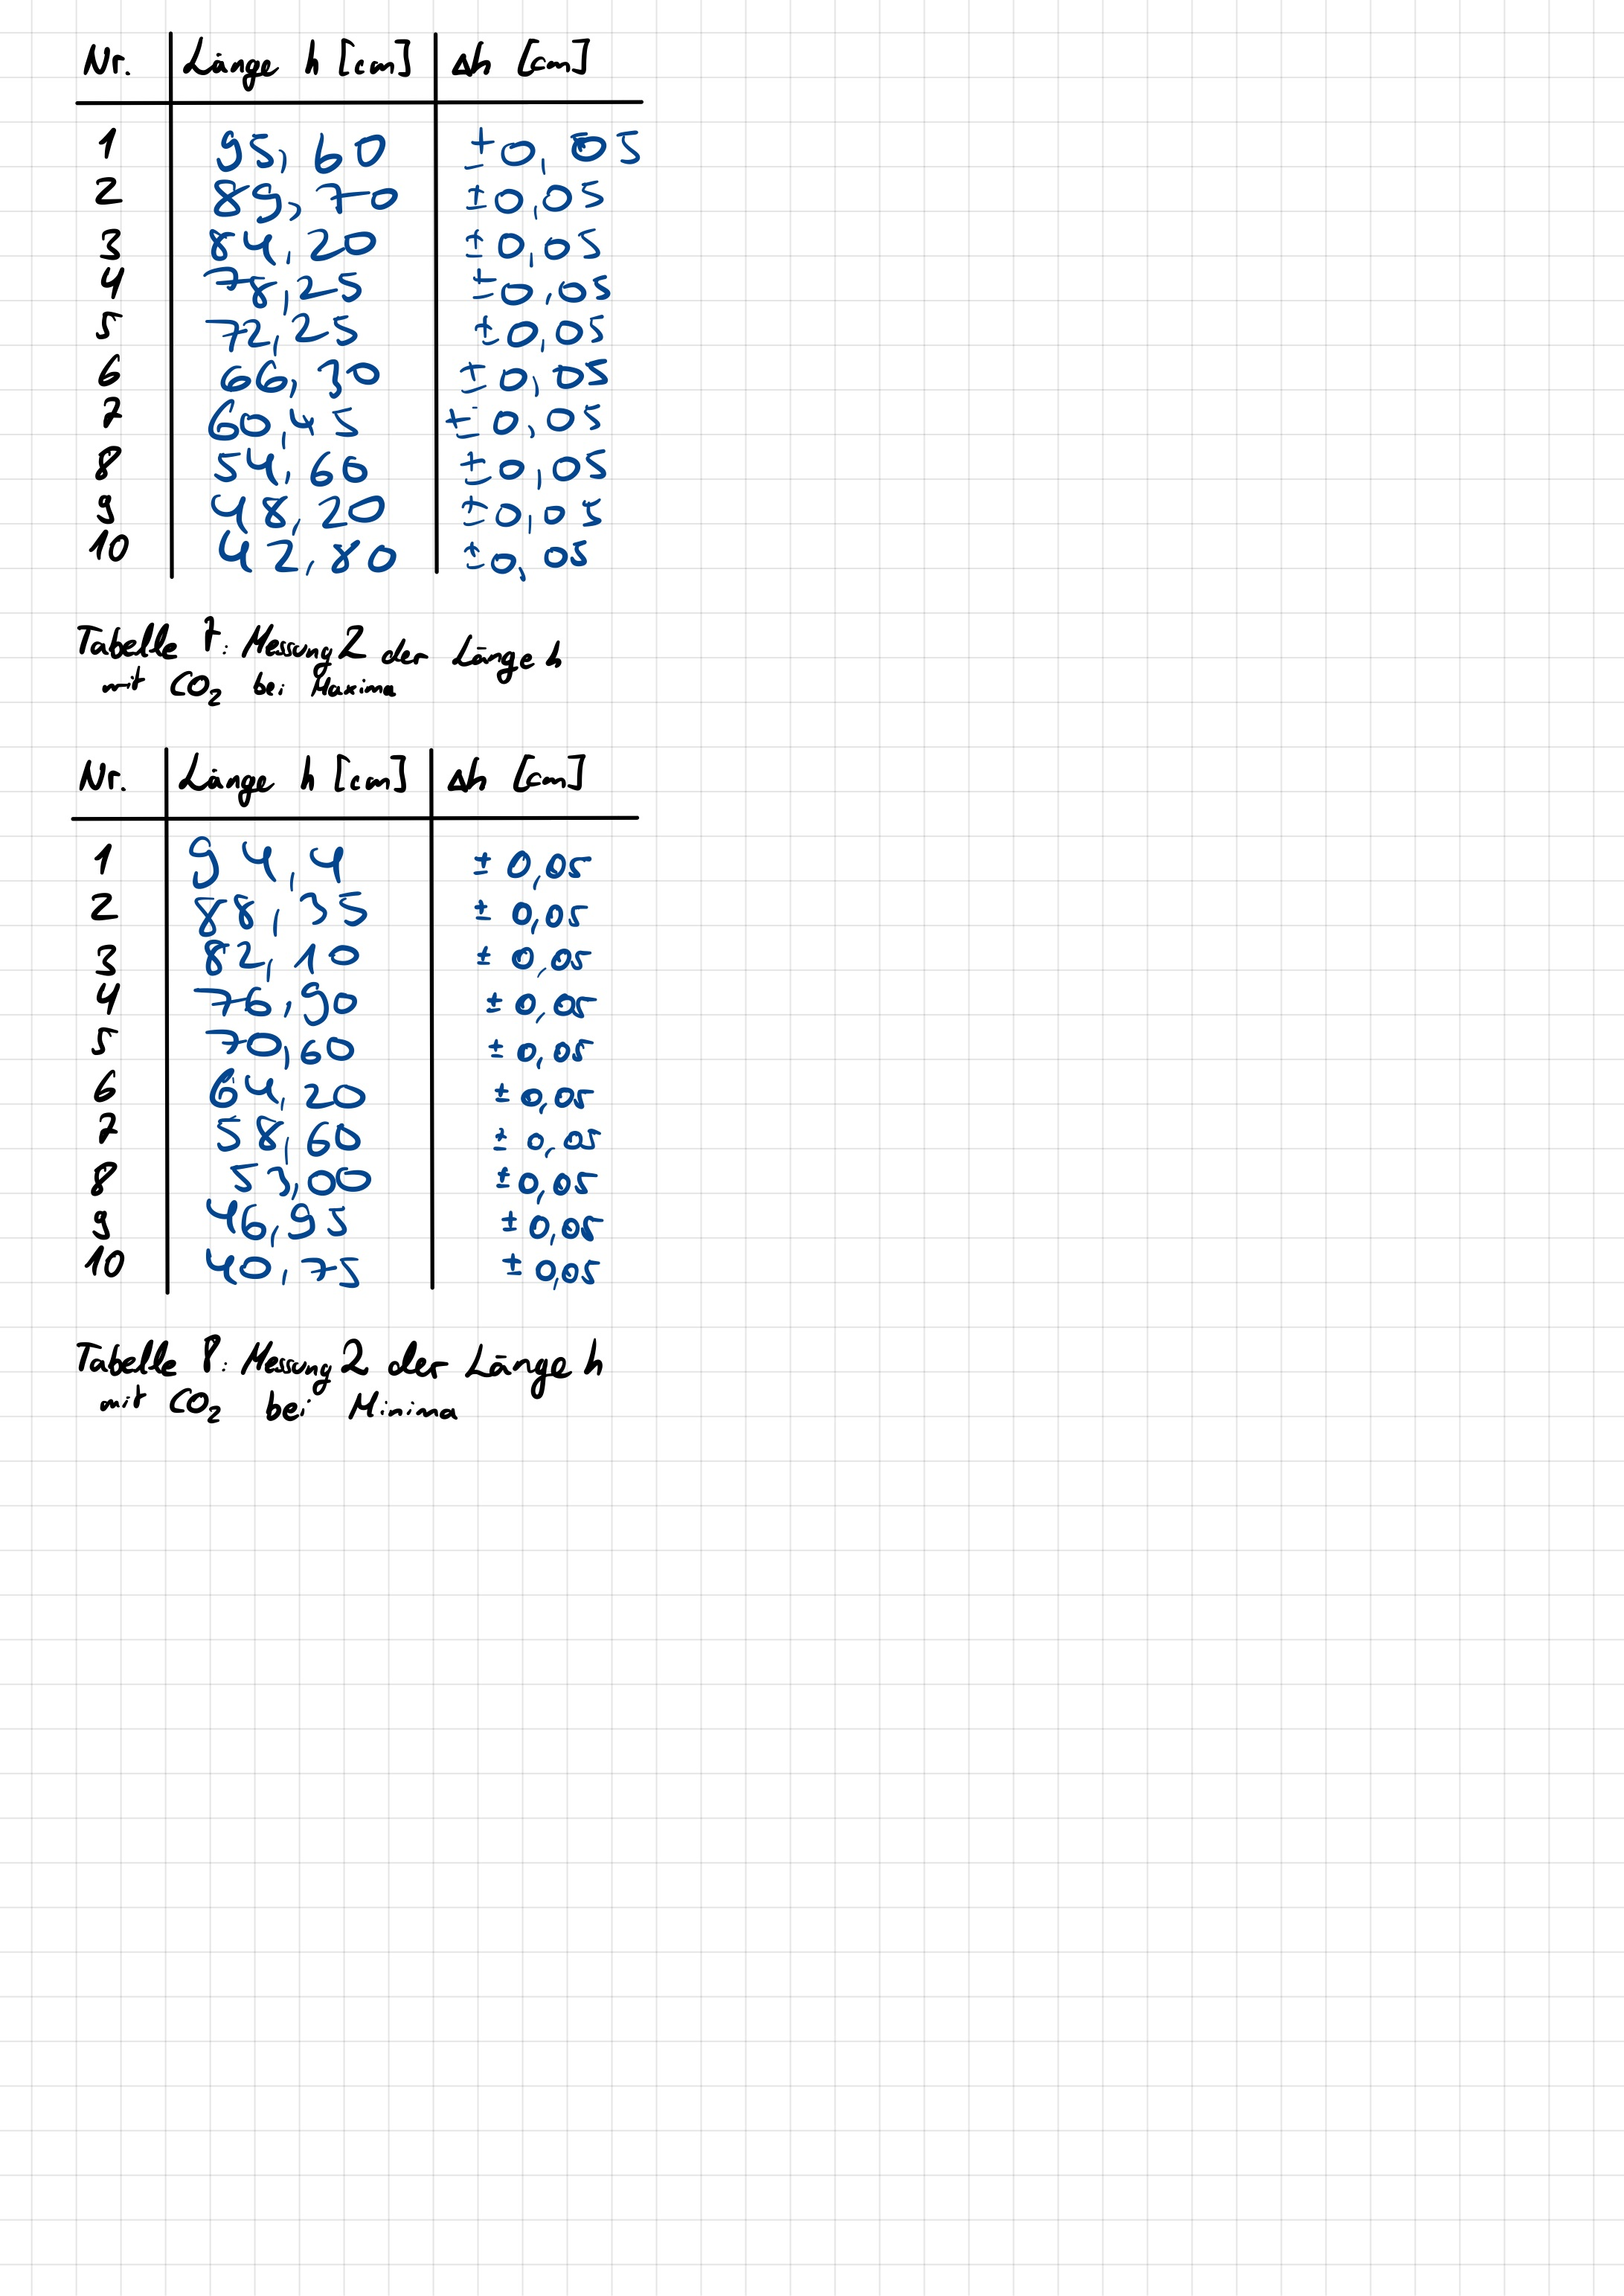
\includegraphics[width=\textwidth]{graphics/mess4.jpg}
\newpage
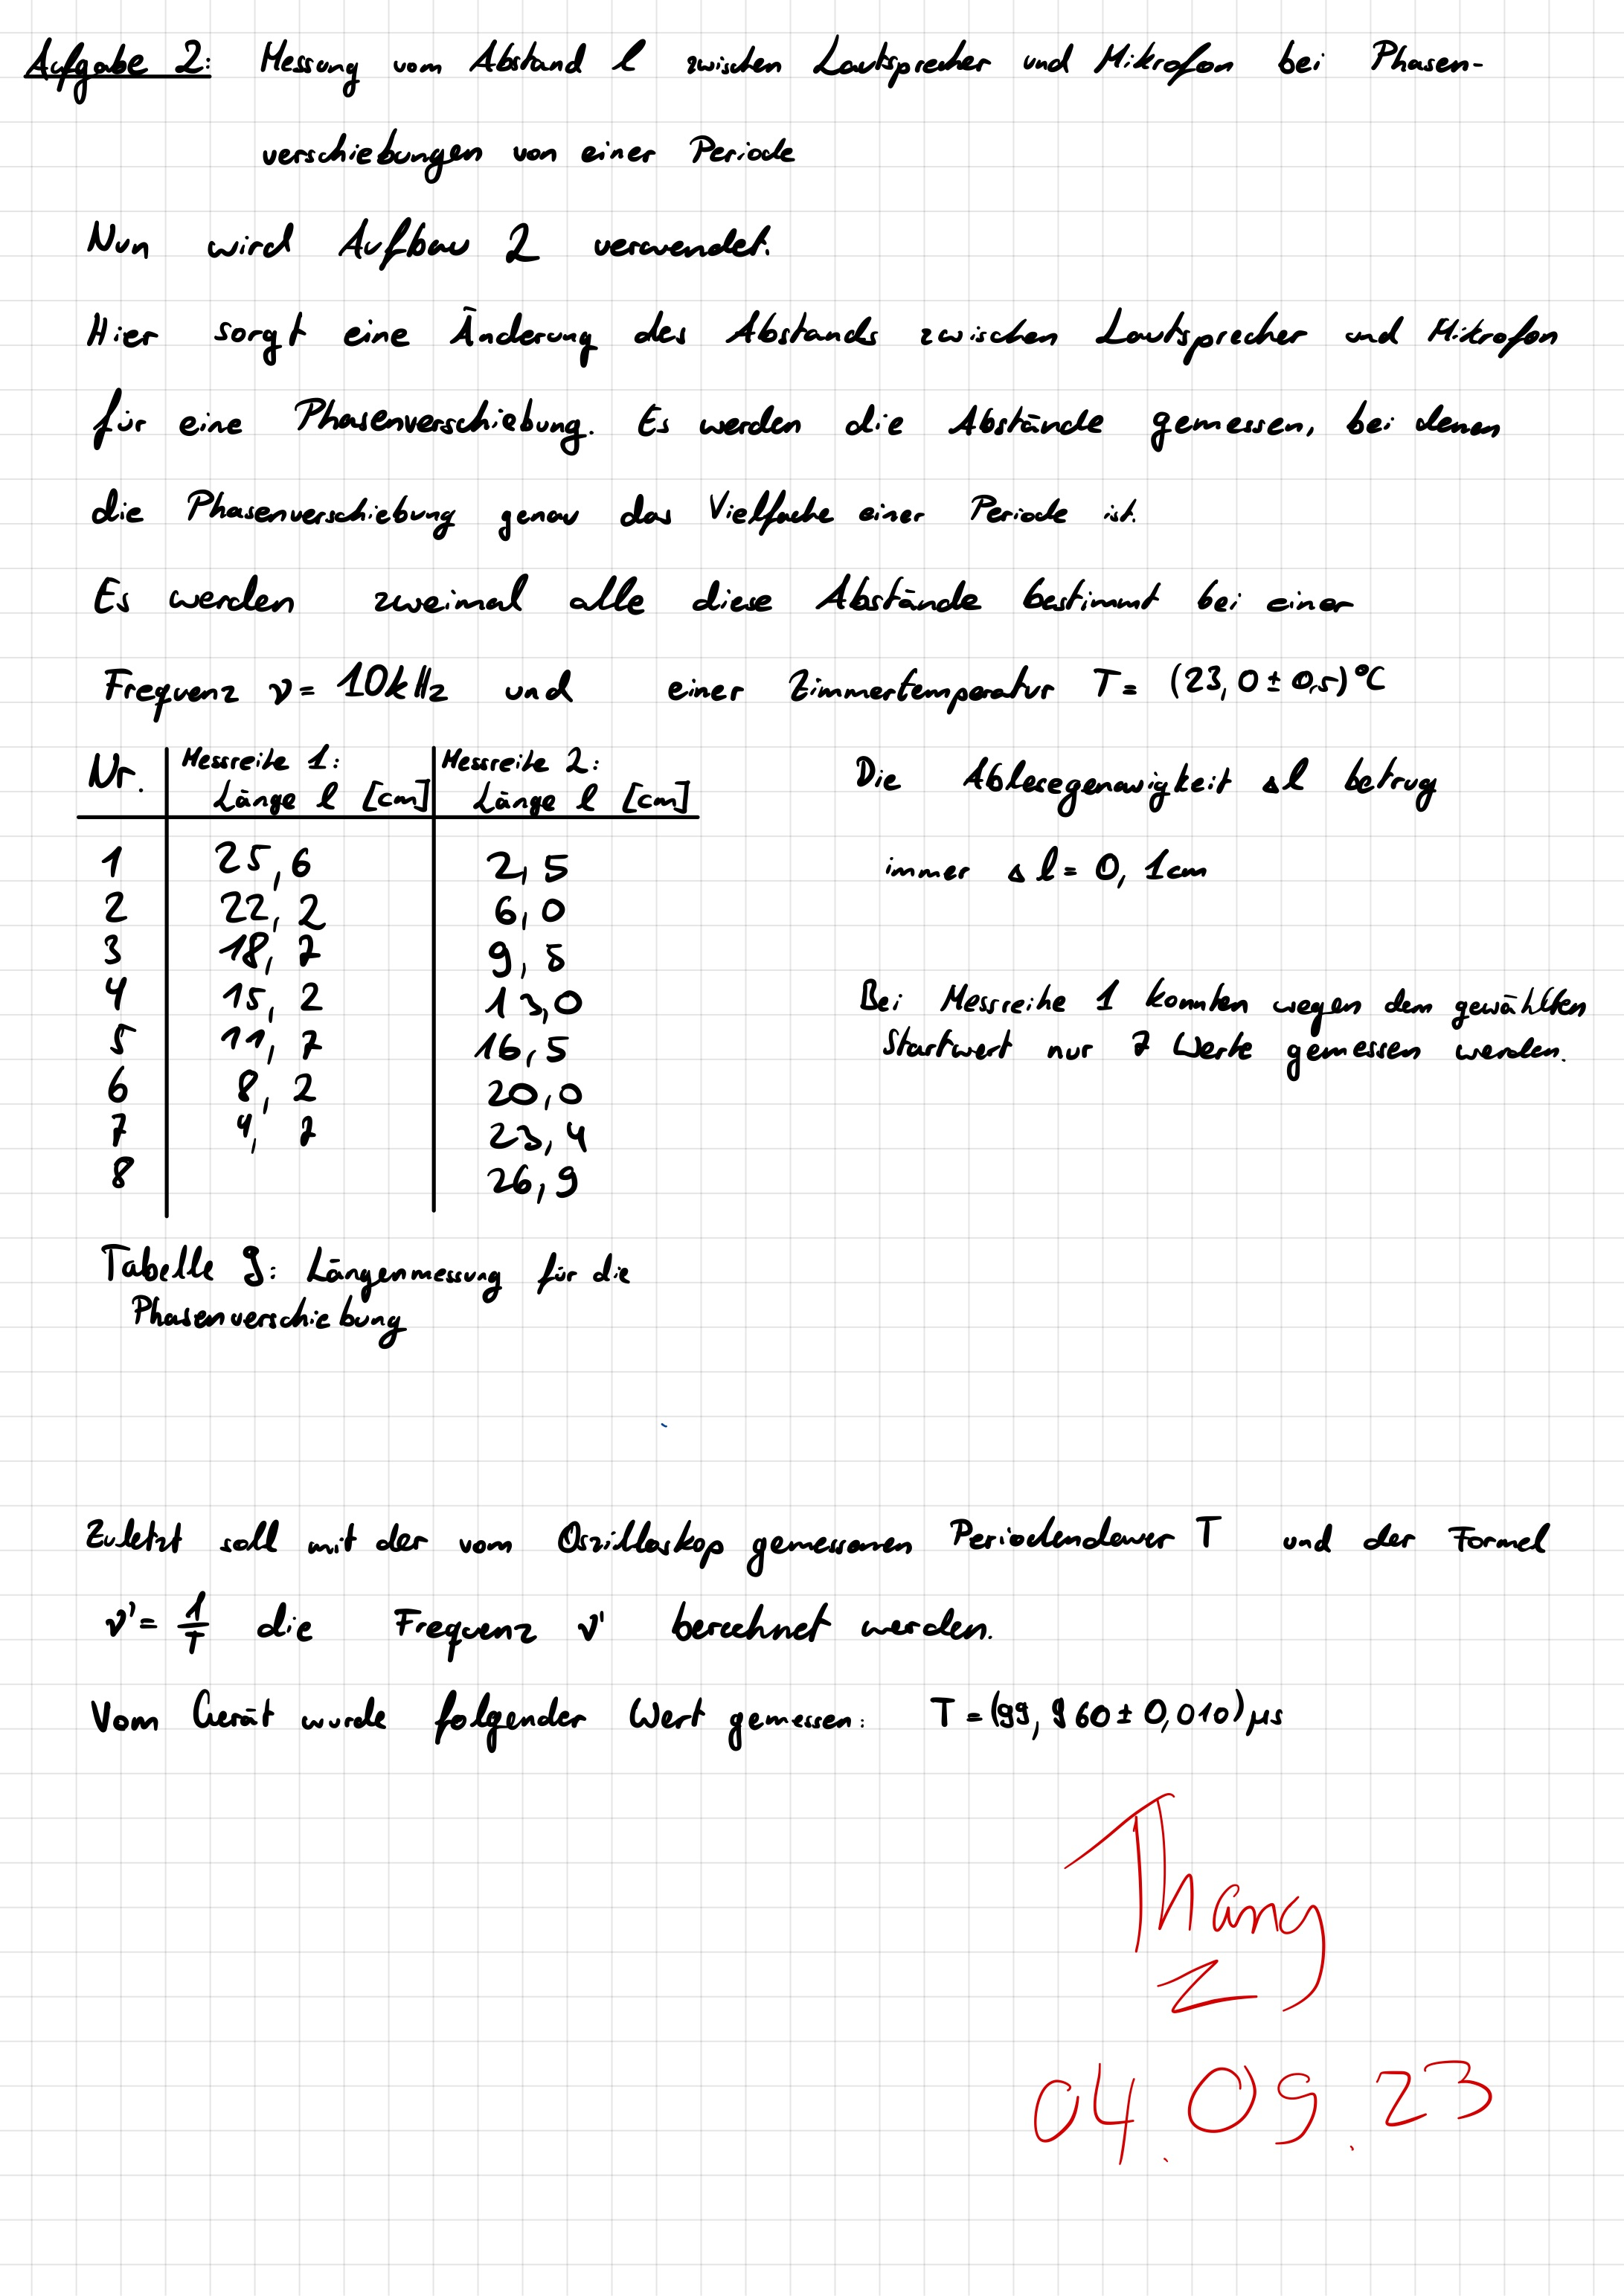
\includegraphics[width=\textwidth]{graphics/mess5.jpg}
\newpage

\addtocounter{table}{9}

%-------------------------AUSWERTUNG-------------------------
\newpage

\section{Auswertung}

\subsection{Zu Aufgabe 1}

Zunächst gilt es, aus den gemessenen Werten die Abstände $D$ zwischen nachfolgenden Werten zu bestimmen. Daraus werden dann Standartabweichung $\sigma_D$, Mittelwert $\overline{D}$ und Standartfehler des Mittelwerts $\Delta \overline{D}_{\sigma}$ bestimmt. 

Die Ergebnisse hierzu sind in Tabelle 10 für Luft und in Tabelle 11 für $CO_2$ zu sehen.

Man berechnet auch den Fehler $\Delta D$ mit Fehlerfortpflanzung und bekommt mit unserer angegeben Messgenauigkeit von $\Delta h = 0,05cm$:

\begin{equation}
    \Delta D = \sqrt{(\Delta h_2)^2+(\Delta h_1)^2} = 0,07cm
\end{equation}

Für den engültigen Fehler des Mittelwerts addiert man nun $\Delta D$ und $\Delta \overline{D}_{\sigma}$ quadratisch und erhält:

\begin{equation}
    \begin{split}
        \Delta \overline{D}_{Luft} &= 0,18cm \\
        \Delta \overline{D}_{CO_2} &= 0,10cm
    \end{split}
\end{equation}

Will man nun die Schallgeschwindigkeit bestimmen, so setzt man die berechneten Werte für $\overline{D}$ sowie den Wert der Frequenz des Sinusgernerators zunächst in Gleichung (3) ein und erhält damit:

\begin{equation}
\begin{split}
    c_{Luft} &= 339,47 \frac{m}{s} \\
    c_{CO_2} &= 271,22 \frac{m}{s}
\end{split}
\end{equation}

Die Fehler berechnen sich nach dem Fehlerfortpflanzungsgesetzt:

\begin{equation}
    \Delta c = \sqrt{(2 \nu \Delta \overline{D})^2 + (2 \overline{D} \Delta \nu )^2}
\end{equation}

Man erhält also:

\begin{equation}
    \begin{split}
        \Delta c_{Luft} &= 8,22 \frac{m}{s} \\
        \Delta c_{CO_2} &= 4,59 \frac{m}{s}
    \end{split}
\end{equation}

Nun kann man diese Werte mit Gleichung (5) und dem gemessenen Wert der Zimmertemperatur $T = (23,0 \pm 0,5)^{\circ}C = (296,7 \pm 0,5)^{\circ}K$ zu den Werten unter Normalbedingungen $T_0 = 273,15^{\circ}K$ umrechnen, man erhält:

\begin{equation}
    \begin{split}
        c_{0_{Luft}} &= 325,75 \frac{m}{s} \\
        c_{0_{CO_2}} &= 260,25 \frac{m}{s}
    \end{split}
\end{equation}

Die Fehler berechnen sich mit

\begin{equation}
    \Delta c_0 = \sqrt{\left( \sqrt{\frac{T_0}{T}} \Delta c \right)^2 + \left(\frac{c}{2T} \sqrt{\frac{T_0}{T}} \Delta T \right)^2}
\end{equation}

zu den Werten

\begin{equation}
    \begin{split}
        \Delta c_{0_{Luft}} &= 7,89 \frac{m}{s} \\
        \Delta c_{0_{CO_2}} &= 4,41 \frac{m}{s} .
    \end{split}
\end{equation}

Berechnet man zum Vergleich die Werte der Schallgeschwindigkeiten mit Gleichung (4) mit den gegebenen Werten so erhält man:

\begin{equation}
    \begin{split}
        c'_{0_{Luft}} &= 331,12 \frac{m}{s} \\
        c'_{0_{CO_2}} &= 259,04 \frac{m}{s}
    \end{split}
\end{equation}

Zum Vergleich werden die Quotienten aus den Geschwindigkeiten berechnet, man erhält:

\begin{equation}
    \begin{split}
        \frac{c'_{0_{Luft}}}{c'_{0_{CO_2}}} &= 1,28 \\
        \frac{c_{0_{Luft}}}{c_{0_{CO_2}}} &= 1,25
    \end{split}
\end{equation}

Der Fehler des zweiten Wertes lässt sich berechnen mit:

\begin{equation}
    \Delta \frac{c_{0_{Luft}}}{c_{0_{CO_2}}} = \frac{c_{0_{Luft}}}{c_{0_{CO_2}}} \sqrt{\left( \frac{\Delta c_{0_{Luft}}}{c_{0_{Luft}}} \right)^2 + \left( \frac{\Delta c_{0_{CO_2}}}{c_{0_{CO_2}}} \right)^2} = 0,04
\end{equation}

Somit liegen das berechnete Verhältnits von $c'_0$ also in den Fehlergrenzen vom berechneten Verhältnis von $c_0$ und man kann sehen, dass die Differenz zwischen den beiden Verhältnissen kleiner ist als der Fehler dieser Differenz, weshalb der Unterschied nicht signifikant ist:

\begin{equation}
    \begin{split}
        \sigma &= \frac{\frac{c'_{0_{Luft}}}{c'_{0_{CO_2}}} - \frac{c_{0_{Luft}}}{c_{0_{CO_2}}}}{\Delta \frac{c_{0_{Luft}}}{c_{0_{CO_2}}}} = 0,75
    \end{split}
\end{equation}

Wir befinden uns also in der $3\sigma$-Umgebung womit der Unterschied nicht signifikant ist.

Zusammenfassend kommen wir also auf folgende Ergebnisse:

\begin{equation}
    \begin{split}
        \bm{c_{0_{Luft}}} &= \bm{(325,75 \pm 7,89) \frac{m}{s}} \\
        \bm{c_{0_{CO_2}}} &= \bm{(260,25 \pm 4,41) \frac{m}{s}} \\
        \bm{c'_{0_{Luft}}} &= \bm{331,12 \frac{m}{s}} \\
        \bm{c'_{0_{CO_2}}} &= \bm{259,04 \frac{m}{s}}
    \end{split}
\end{equation}

\begin{table}[p]
    \centering
    \caption{Auswertung der Messergebnisse bei Luft von Aufgabe 1}
    \begin{tabular}{c|c|c|c|c|c}
        Tabellennr. & Messnr. & $D$ [cm] & $\overline{D}_{Luft}$ [cm] & $\sigma_{D_{Luft}}$ [cm] & $\Delta \overline{D}_{\sigma_{Luft}}$ [cm] \\ \hline
        1 & 1-2 & 9,50 & 7,46 & 1,026 & 0,17 \\
        1 & 2-3 & 7,20 &  &  & \\
        1 & 3-4 & 8,00 &  &  & \\
        1 & 4-5 & 7,50 &  &  & \\
        1 & 5-6 & 7,70 &  &  & \\
        1 & 6-7 & 7,55 &  &  & \\
        1 & 7-8 & 7,40 &  &  & \\
        1 & 8-9 & 7,85 &  &  & \\
        1 & 9-10 & 7,60 &  &  & \\ \cline{1-3}
        2 & 1-2 & 4,90 &  &  & \\
        2 & 2-3 & 7,60 &  &  & \\
        2 & 3-4 & 9,80 &  &  & \\
        2 & 4-5 & 5,80 &  &  & \\
        2 & 5-6 & 9,20 &  &  & \\
        2 & 6-7 & 7,90 &  &  & \\
        2 & 7-8 & 4,30 &  &  & \\
        2 & 8-9 & 7,90 &  &  & \\
        2 & 9-10 & 8,00 &  &  & \\ \cline{1-3}
        3 & 1-2 & 7,70 &  &  & \\
        3 & 2-3 & 7,50 &  &  & \\
        3 & 3-4 & 7,80 &  &  & \\
        3 & 4-5 & 7,50 &  &  & \\
        3 & 5-6 & 7,55 &  &  & \\
        3 & 6-7 & 7,50 &  &  & \\
        3 & 7-8 & 7,80 &  &  & \\
        3 & 8-9 & 7,55 &  &  & \\
        3 & 9-10 & 7,20 &  &  & \\ \cline{1-3}
        4 & 1-2 & 7,30 &  &  & \\
        4 & 2-3 & 7,30 &  &  & \\
        4 & 3-4 & 8,10 &  &  & \\
        4 & 4-5 & 7,90 &  &  & \\
        4 & 5-6 & 6,60 &  &  & \\
        4 & 6-7 & 7,55 &  &  & \\
        4 & 7-8 & 6,80 &  &  & \\
        4 & 8-9 & 6,65 &  &  & \\
        4 & 9-10 & 6,60 &  &  &  
\end{tabular}
\end{table}

\begin{table}[p]
    \centering
    \caption{Auswertung der Messergebnisse bei $CO_2$ von Aufgabe 1}
    \begin{tabular}{c|c|c|c|c|c}
        Tabellennr. & Messnr. & $D$ [cm] & $\overline{D}_{CO_2}$ [cm] & $\sigma_{D_{CO_2}}$ [cm] & $\Delta \overline{D}_{\sigma_{CO_2}}$ [cm] \\ \hline
        5 & 1-2 & 6,40 & 5,96 & 0,46 & 0,07 \\
        5 & 2-3 & 5,05 &  &  & \\
        5 & 3-4 & 6,50 &  &  & \\
        5 & 4-5 & 6,20 &  &  & \\
        5 & 5-6 & 5,50 &  &  & \\
        5 & 6-7 & 6,15 &  &  & \\
        5 & 7-8 & 6,35 &  &  & \\
        5 & 8-9 & 5,30 &  &  & \\
        5 & 9-10 & 6,50 &  &  & \\ \cline{1-3}
        6 & 1-2 & 5,25 &  &  & \\
        6 & 2-3 & 6,80 &  &  & \\
        6 & 3-4 & 6,25 &  &  & \\
        6 & 4-5 & 6,45 &  &  & \\
        6 & 5-6 & 5,60 &  &  & \\
        6 & 6-7 & 5,15 &  &  & \\
        6 & 7-8 & 6,10 &  &  & \\
        6 & 8-9 & 5,75 &  &  & \\
        6 & 9-10 & 6,65 &  &  & \\ \cline{1-3}
        7 & 1-2 & 5,90 &  &  & \\
        7 & 2-3 & 5,50 &  &  & \\
        7 & 3-4 & 5,95 &  &  & \\
        7 & 4-5 & 6,00 &  &  & \\
        7 & 5-6 & 5,95 &  &  & \\
        7 & 6-7 & 5,85 &  &  & \\
        7 & 7-8 & 5,85 &  &  & \\
        7 & 8-9 & 6,40 &  &  & \\
        7 & 9-10 & 5,40 &  &  & \\ \cline{1-3}
        8 & 1-2 & 6,05 &  &  & \\
        8 & 2-3 & 6,25 &  &  & \\
        8 & 3-4 & 5,20 &  &  & \\
        8 & 4-5 & 6,30 &  &  & \\
        8 & 5-6 & 6,40 &  &  & \\
        8 & 6-7 & 5,60 &  &  & \\
        8 & 7-8 & 5,60 &  &  & \\
        8 & 8-9 & 6,05 &  &  & \\
        8 & 9-10 & 6,20 &  &  &  
\end{tabular}
\end{table}

\newpage

\subsection{Zu Aufgabe 2}

Zunächst werden aus den in Tabelle 9 gemessenen Werten erneut die Differenzen und deren Mittelwert sowie dessen Fehler berechnet. 

Die Ergebnisse dazu sind in Tabelle 12 festgehalten.

\begin{table}[h]
    \centering
    \caption{Auswertung der Messergebnisse von Aufgabe 2}
    \begin{tabular}{c|c|c|c|c|c}
        Messreihe & Messnr. & $D$ [cm] & $\overline{D}$ [cm] & $\sigma_{D}$ [cm] & $\Delta \overline{D}_{\sigma}$ [cm] \\ \hline
        1 & 1-2 & 3,4 & 3,48 & 0,03 & 0,01 \\
        1 & 2-3 & 3,5 &  &  & \\
        1 & 3-4 & 3,5 &  &  & \\
        1 & 4-5 & 3,5 &  &  & \\
        1 & 5-6 & 3,5 &  &  & \\
        1 & 6-7 & 3,5 &  &  & \\ \cline{1-3}
        2 & 1-2 & 3,5 &  &  & \\
        2 & 2-3 & 3,5 &  &  & \\
        2 & 3-4 & 3,5 &  &  & \\
        2 & 4-5 & 3,5 &  &  & \\
        2 & 5-6 & 3,5 &  &  & \\
        2 & 6-7 & 3,4 &  &  & \\
        2 & 7-8 & 3,5 &  &  & 
\end{tabular}
\end{table}

Der Fehler von $D$ lässt sich auch wieder analog zu Gleichung (9) berechnen, hier hat man nur kein $\Delta h$ sondern ein $\Delta l$, und man bestimmt den Mittelwertsfehler auch analog:

\begin{equation}
    \begin{split}
        \Delta D &= 0,14 cm \\
        \Delta \overline{D} &= 0,14cm
    \end{split}
\end{equation}

%Da dieser Wert größer ist als $\sigma_{D}$ muss dieser nun verwendet werden und es berechnet sich ein neues $\Delta \overline{D}'$ zu

%\begin{equation}
    %\Delta \overline{D}' = \frac{\Delta D}{\sqrt{13}} = 0,04 cm
%\end{equation}

Man berechnet die Schallgeschwindigkeit nun gemäß Gleichung (8) zu

\begin{equation}
    c = \nu \overline{D} = 348 \frac{m}{s}
\end{equation}
 und den Fehler gemäß dem Fehlerfortpflanzungsgesetzes zu

\begin{equation}
    \Delta c = \sqrt{(\nu \Delta \overline{D})^2} = 14 \frac{m}{s} .
\end{equation}

Nun rechnet man das Ergebnis noch auf Normalbedingungen um und erhält:

\begin{equation}
    \begin{split}
        c_0 &= 333,9 \frac{m}{s} \\
        \Delta c_0 &= 13,4 \frac{m}{s} \\
        \bm{c_0} &= \bm{(333,9 \pm 13,4) \frac{m}{s}}
    \end{split}
\end{equation}

Vergleicht man dieses Ergebnis mit dem berechneten Wert für $c'_{0_{Luft}}$ und berechnet wieder die Differenz $x$ mit Fehler $\Delta x$ so erhält man:

\begin{equation}
    \begin{split}
        x &= 2,78 \frac{m}{s} \\
        \Delta x &= 13,4 \frac{m}{s} \\ \\
        \implies \sigma &= \frac{x}{\Delta x} = 0,21
    \end{split}
\end{equation}

Der Unterschied ist also auch hier nicht signifikant.

%---------------PRÄSENTATION DER ENDERGEBNISSE---------------
\newpage

\section{Präsentation der Endergebnisse}

Zusammenfassend wurden bei diesem Versuch die folgenden Ergebnisse erziehlt.

Die genauesten Werte wurde Mithilfe der Formel für die Schallgeschwindikeit in Gasen bestimmt als:

\begin{equation}
    \begin{split}
        \bm{c'_{0_{Luft}} = 331,12 \frac{m}{s}} \\
        \bm{c'_{0_{CO_2}} = 259,04 \frac{m}{s}}
    \end{split}
\end{equation}

Bei der Bestimmung der Schallgeschwindigkeit mit dem Quinke'schen Rohr wurden folgende Werte bestimmt:

\begin{equation}
    \begin{split}
        \bm{c_{0_{Luft}}} &= \bm{(325,75 \pm 7,89) \frac{m}{s}} \\
        \bm{c_{0_{CO_2}}} &= \bm{(260,25 \pm 4,41) \frac{m}{s}} 
    \end{split}
\end{equation}

Zuletzt wurde über die Laufzeitmessung der Wert der Schallgeschwindigkeit in Luft ermittelt als:

\begin{equation}
        \bm{c_0 = (333,9 \pm 13,4) \frac{m}{s}}
\end{equation}

%---------------ZUSAMMENFASSUNG UND DISKUSSION---------------
\newpage

\section{Zusammenfassung und Diskussion}

In diesem Versuch wurde auf zwei verschiedenen Wegen die Schallgeschwindigkeit bestimmt. Im ersten Versuchsteil wurde eine stehende Welle im Quinke'schen Rohr auf ihre Maxima und Minima in Abhängigkeit vom Wasserstand im Rohr untersucht, während im zweiten Teil mithilfe eines Oszilloskops eine Laufzeitmessung durchgeführt wurde, bei der wir die Entfernung eines Lautsprechers zu einem Mikrofon variierten, sodass die Schallwelle um genau eine Periode verschoben wurde. 

Was bei der Auswertung zunächst Positiv auffällt ist, dass alle berechneten Werte für die Schallgeschwindigkleiten in Luft und $CO_2$ nicht signifikant vom berechneten Idealwert abweichen. Ein wichtiger Faktor waren hier sicherlich die Ergebnisse vom ersten Aufgabenteil, wo wir nicht nur die von der Aufgabenstellung geforderten Maxima, sondern auch immer die Minima bestimmt haben, was dazu führte, dass wir die doppelte Anzahl an Messwerten zur Verfügung hatten. Dies minimierte schonmal den statistischen Fehler in der Auswertung. 

Hier lässt sich allerdings auch der erste Optimierungsvorschlag nennen. Da der erste Versuchsteil darauf aufbaut, dass man selbst die Maxima und Minima hört, war die Versuchsumgebung nicht optimal. Störende Geräusche im Hintergrund, wie beispielsweise die Töne der Lautsprecher für die Experimente der anderen Gruppen, waren fast immer ein nicht vermeidbares Hindernis, besonders bei der Bestimmung der Minimapositionen. Auch lässt sich allgemein der Hörfehler nennen, da die Lautstärke rein nach eigenem Ermessen bestimmt wurde, was nicht zwangsläufig präzise sein muss. Ein weitere Punkt beim ersten Teil war, dass der benutzte Sinusgenerator bei allen drei verfügbaren Versuchsaufbauten keine konstante Frequenz lieferte. Der Wert fiel bei uns immer mit der Zeit langsam ab, was auch zum angegeben Fehler der Frequenz führte und somit auch den endgültigen Wert beeinflusst. Speziell zur Messung an der mit $CO_2$ gefüllten Röre lässt sich noch sagen, dass zum einen das Entweichen des Gases aus dem Rohr immer eine mögliche Fehlerquelle sein kann und zum anderen das Einfüllen des Gases immer zu einem Aufsprudeln des Wassers gefüht hat, wodurch sich Wassertropfen an der Rohrinnenseite bildeten, die zum Teil die Sicht auf die Messkala hinter dem Rohr erschwerten. 

Beim zweiten Versuchsteil ist zunächst anzumerken, dass wir bei der ersten Messreihe einen ungünstigen Startwert gewählt hatten, weshalb wir nur 7 anstatt 8 Positionen bestimmen konnten. Ein besser gewählter Startwert oder sogar eine dritte Messreihe hätten hier sicherlich geholfen. Auffallend groß ist hier auch der Fehler der am Ende bestimmten Schallgeschwindigkeit von $13,4 \frac{m}{s}$. Ein großer Beitrag hierzu wird wohl der Ablesefehler sein, den wir als $\Delta l = 0,1cm$ angegeben haben, während wir beim ersten Versuchsteil nur einen Fehler von $\Delta h = 0,05cm$ abgeschätzt hatten.

Allgemeine Fehler sind natürlich auch immer trotz Angabe die Ablesegenauigkeit sowie die Gerätefehler. Bis auf den selbst bestimmten Wert aufgrund der Schwankung des Sinusgenerators beim ersten Versuchsteil standen aber keine Gerätefehler zur Verfügung. 

Zum Schluss lässt sich das Fazit ziehen, dass trotz den genannten potenziellen Fehlerquellen alle Werte ohne signifikante Abweichungen bestimmt werden konnten, was als ein positives Ergebnis dieses Versuchs gesehen werden kann. 

\end{document}

